\chapter{Proje Dosya Yapısı ve Mimari}

\noindent
% -------------------------------------------------------------------------
% SOL KOLON (Görsel ve Sheet Mantığı)
% -------------------------------------------------------------------------
\begin{minipage}[t]{0.48\textwidth}
    {\Large \bfseries \textcolor{primary}{VBA Proje Ağacı}} \\[0.15cm]
    \small Projede yer alan tüm dosya, modül ve sınıf yapıları katmanlı mimari (\textit{Layered Architecture}) prensiplerine uygun kurgulanmıştır.

    \vspace{0.25cm}

    % Proje Ağacı Görseli
    \centering
    \fboxsep=0pt
    \fboxrule=0.5pt
    \fcolorbox{bordergray}{white}{%
        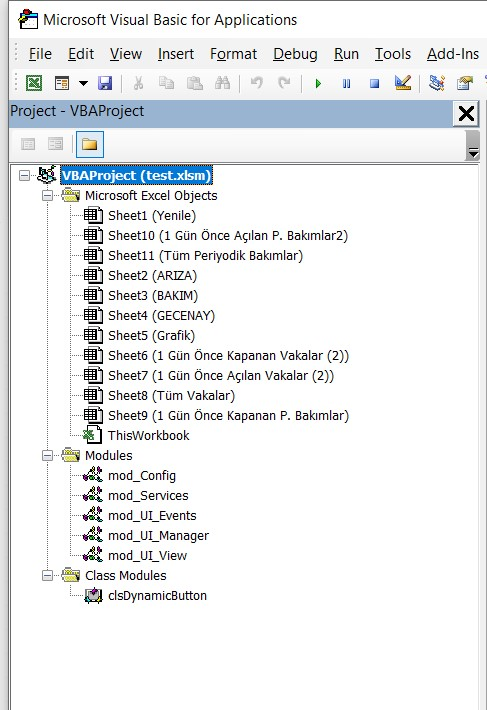
\includegraphics[width=0.90\linewidth, height=7.5cm, keepaspectratio]{project_files.jpg}%
    }
    \captionof{figure}{VBA Proje Ağacı}

    \vspace{0.3cm}

    \begin{tcolorbox}[colback=lightgray,colframe=bordergray,leftrule=3.5pt,boxrule=0.4pt,top=4.5pt,bottom=4.5pt]
        \textbf{\textcolor{primary}{\faFileExcel\ Excel Sheet Modülleri:}}\\
        \small Projede yer alan \textbf{Sheet1 (Yenile)}, \textbf{Sheet2 (ARIZA)}, \textbf{Sheet3 (BAKIM)} ve \textbf{Sheet4 (GECENAY)} gibi yerleşik sayfaların içerisine kod yazılmamıştır. 

        Kolay okunur kod yapısı sağlamak amacıyla tüm olaylar servis katmanına yönlendirilmiştir.
    \end{tcolorbox}
    
    \vspace{0.15cm}

    \begin{tcolorbox}[colback=lightgray,colframe=bordergray,leftrule=3.5pt,boxrule=0.4pt,top=4.5pt,bottom=4.5pt]
        \textbf{\textcolor{primary}{\faBook\ ThisWorkbook:}}\\
        \small Çalışma kitabı açılış/kapanış olaylarını (\texttt{Workbook\_Open}) ve sistem ilklendirme süreçlerini yönetir.
    \end{tcolorbox}
\end{minipage}
\hfill
% -------------------------------------------------------------------------
% SAĞ KOLON (Modüller ve Class)
% -------------------------------------------------------------------------
\begin{minipage}[t]{0.48\textwidth}
    {\Large \bfseries \textcolor{primary}{Standart Modüller}} \\[0.2cm]

    \begin{tcolorbox}[colback=lightgray,colframe=bordergray,leftrule=3pt,boxrule=0.4pt,top=4.5pt,bottom=4.5pt]
        \textbf{\textcolor{primary}{\faCog\ mod\_Config:}}\\
        \small Sabitler (Constants), renk kodları, hücre adresi eşleşmeleri ve konfigürasyon değişkenlerini barındırır.
    \end{tcolorbox}

    \begin{tcolorbox}[colback=lightgray,colframe=bordergray,leftrule=3pt,boxrule=0.4pt,top=4.5pt,bottom=4.5pt]
        \textbf{\textcolor{primary}{\faServer\ mod\_Services:}}\\
        \small Veri arama, tarih doğrulamaları ve arka plan hesaplamalarını yürüten ana iş mantığı (Business Logic) katmanıdır.
    \end{tcolorbox}

    \begin{tcolorbox}[colback=lightgray,colframe=bordergray,leftrule=3pt,boxrule=0.4pt,top=4.5pt,bottom=4.5pt]
        \textbf{\textcolor{primary}{\faMousePointer\ mod\_UI\_Events:}}\\
        \small Kullanıcı etkileşimleri ve sayfa içi olay yönlendirmelerini dinleyen event modülüdür.
    \end{tcolorbox}

    \begin{tcolorbox}[colback=lightgray,colframe=bordergray,leftrule=3pt,boxrule=0.4pt,top=4.5pt,bottom=4.5pt]
        \textbf{\textcolor{primary}{\faSlidersH\ mod\_UI\_Manager:}}\\
        \small Arayüz elemanlarının koordinasyonu ve oturum durumlarının yönetildiği katmandır.
    \end{tcolorbox}

    \begin{tcolorbox}[colback=lightgray,colframe=bordergray,leftrule=3pt,boxrule=0.4pt,top=4.5pt,bottom=4.5pt]
        \textbf{\textcolor{primary}{\faPaintBrush\ mod\_UI\_View:}}\\
        \small Dinamik panellerin çizimi ve görsel bileşenlerin sayfaya basılmasından sorumlu arayüz katmanıdır.
    \end{tcolorbox}

    \vspace{0.4cm}

    {\Large \bfseries \textcolor{primary}{Sınıf Modülleri}} \\[0.2cm]

    \begin{tcolorbox}[colback=lightgray,colframe=bordergray,leftrule=3.5pt,boxrule=0.4pt,top=4.5pt,bottom=4.5pt]
        \textbf{\textcolor{primary}{\faCube\ clsDynamicButton:}}\\
        \small Sayfa üzerinde çalışma zamanında (runtime) dinamik olarak oluşturulan butonların tıklanma olaylarını (Event-Handling) nesne tabanlı olarak yöneten sınıf yapısıdır.
    \end{tcolorbox}
\end{minipage}